\section{Ethereum Heuristics} 
\label{sec:eth}

Using this large dataset, we describe two Ethereum-wide heuristics used to cluster together addresses potentially belonging to the same entity.
 % After summarizing each algorithm, we will present key advantages and drawbacks.

\subsection{Deposit Address Reuse}
\label{sec:dar}

Deposit address reuse (DAR) links together EOAs through the usage of a centralized exchange (CEX). We refer to the original paper \citep{victor2020address} for a detailed description but provide an overview here.

\begin{figure}[b!]
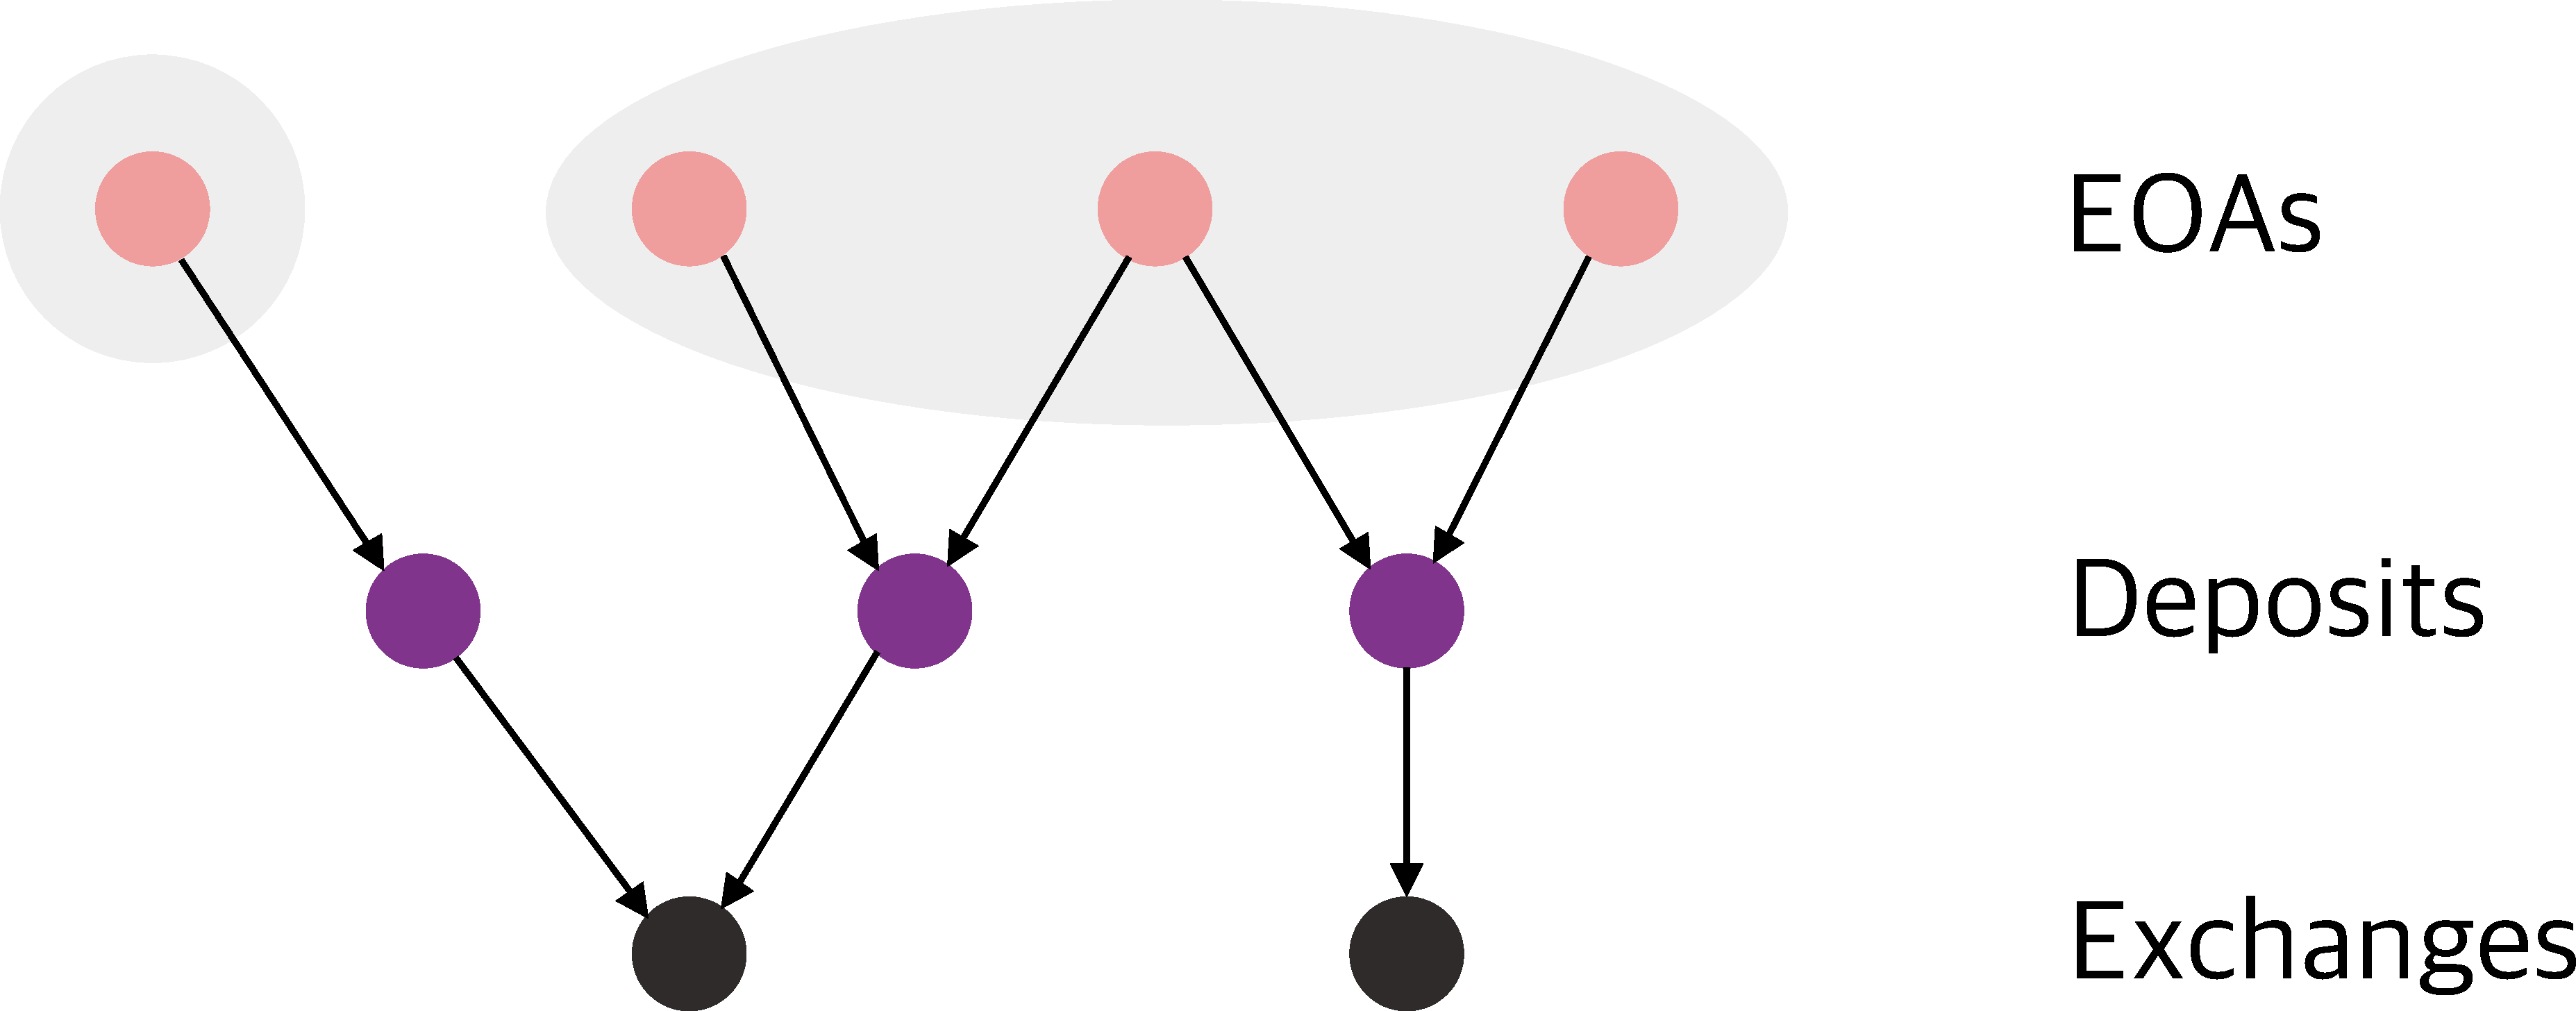
\includegraphics[width=\linewidth]{figures/dar.pdf}
\caption{Graph of transactions between EOA, deposit, and CEX addresses. A cluster is defined as a weakly connected component in an undirected subgraph containing only EOA and deposit nodes. The gray circles show EOA addresses in two clusters.}
\label{fig:dar}
\end{figure}

When users sell Ether to a CEX, the exchange typically creates ``deposit addresses'', which receive the assets from the EOA and then forward these funds to the main address associated with the CEX. Critically, these deposit addresses are created per customer, not per address. That is, multiple addresses that send funds to the same deposit address are highly likely to be owned by the same entity. However, these deposit addresses are not known. The DAR algorithm seeks to identify deposit addresses through heuristics.
It uses two hyperparameters: the maximum amount difference $\alpha$ and the maximum time difference $\tau$ between two transactions: a ``receiving'' transaction from an EOA to a suspected deposit address, and a ``forwarding'' transaction from a deposit to a main exchange address (we assume access to a list of main CEX addresses). The intuition is that true deposits likely forward funds quickly, and differences in amount should only be due to transaction fees. We exclude known entities (e.g. CEX, DEX, miner, etc.) from being classified as deposit addresses.

Then, we can search for $($EOA, deposit, exchange$)$ tuples that match the constraints set by $\alpha$ and $\tau$.
If we construct an undirected graph with addresses as nodes and edges between associated EOA and deposits, a ``cluster'' is defined as a weakly connected component. This definition captures interesting cases where a single entity has multiple EOAs that send to different deposits of multiple CEXs (see Figure~\ref{fig:dar}). In practice, we pick $\alpha = 0.01$ and $\tau = 3,200$ \citep{victor2020address}.

For each cluster, we would like to assign a confidence score, representing our belief in this cluster representing a single entity. We note that any uncertainty in clustering must come from uncertainty in defining deposit addresses. So, for any address in a cluster $C$, we assign  confidence as the average confidence for deposits in $C$. Now, for any deposit $v$, we define confidence as:
\begin{equation*}
\kappa(v) = 1 - \left\{ \frac{1}{2}\left(\frac{|a_f - a_r|}{\alpha}\right) + \frac{1}{2}\left(\frac{t_f - t_r}{\tau}\right) \right\}
\end{equation*}
where $a_f$ and $a_r$ are the amounts from the forwarding and receiving transactions, respectively. Similarly, $t_f$ and $t_r$ are the forwarding and receiving block numbers.
A larger difference in either amount or time would decrease the confidence, which is bound to be between 0 and 1.

\subsection{Learned Node Embedding}

The benefit of DAR is interpretability: we can understand (to a degree) why the algorithm believes two addresses are linked. However, this comes at the cost of recall and the ability to identify dense clusters. DAR searches for a very specific behavior, and most addresses will not be in a cluster of greater than size 1. Initial feedback from Tutela users reported limited success in finding clusters.
To supplement DAR, we consider a second Ethereum-wide heuristic (NODE) that projects addresses to points in a low-dimensional vector space based on who it transacts with. In this vector space, addresses belonging to the same entity should be close together in Euclidean distance.

Consider constructing an undirected graph $G(V, E)$ from all Ethereum transactions, where nodes $V$ are composed of distinct addresses, and an edge is placed between two nodes if there is a transaction between them. Each edge is given a weight $w: V \times V \rightarrow \mathbb{N}$ designating the number of interactions between two addresses. For instance, and if Alice has sent Bob 1 ETH five times,  then $w(\textup{Alice}, \textup{Bob}) = 5$. Note that this graph is distinct from the one used in Section~\ref{sec:dar}.

At this abstraction layer, we seek to learn a ``node embedding function'' $f: V \rightarrow \mathbb{R}^d$ that projects a node to a $d$-dimensional vector representation. Importantly, we want this embedding to capture semantic information about the node, such as which other addresses it frequently interacts with. To do so, we leverage popular graph representation learning algorithms \citep{grover2016node2vec,rozemberczki2018fast}. In particular, we focus on Diff2Vec \citep{rozemberczki2018fast}, which has been applied to blockchain transactions \citep{beres2021blockchain}, though not at scale.

The intuition of Diff2Vec is to summarize a node by its neighborhood through a diffusion-like random process. Specifically, there are four steps to Diff2Vec: (1) generating a ``diffusion graph'', (2) sampling a ``node sequence'', (3) extracting features, (4) learning a neural network embedding. We briefly summarize each step below.

\paragraph{Step One} Fixing a starting node $v \in V$, we initialize a diffusion subgraph $\tilde{G}$ containing only $\{v\}$. Randomly sample two nodes, $u$ from $\tilde{G}$ and $w \in \textup{Neighbors}(u, G)$, where $G$ is the original graph. Add node $w$ and the edge $(u, w)$ to $\tilde{G}$. Repeat until $\tilde{G}$ has $l$ nodes, where $l$ is a hyperparameter representing the amount of information we want to capture in our eventual node embedding. A larger $l$ may capture a large neighborhood but sacrifice in granularity.

\paragraph{Step Two} Given $\tilde{G}$, we generate a sequence $s = (v_1, v_2, \ldots)$ recording the nodes visited during an Euler walk. To do this, we must ensure that $\tilde{G}$ is Eulerian, which holds if every node has an even degree. A simple way to achieve this is to double each edge in $\tilde{G}$. At this point, we can summarize a node $v \in V$ by multiple sequences $S = (s_1, s_2, \ldots)$, each from a random walk.

\paragraph{Step Three} Given a set of sequences $S$, we aim to produce a single feature vector based on frequencies of which vertices appear near each other in sequences $s \in S$. Specifically, fix a node $v$. Then, pick a window size $h$.
Count how many times other nodes appear within $h$ positions before and after when $v$ appears, summed over all sequences $s \in S$. This will result in $2h$ vectors each of length $|V|$ --- $2$ from counting before \textit{and} after; $h$ from counting frequencies 1 to $h$ positions away from $v$; $|V|$ since each vector stores counts of all nodes in $V$. Denote this feature vector by $y(v) \in \mathbb{R}^{2h|V|}$.

\paragraph{Step Four} Finally, we wish to compress the feature vector from Step Three to a $d$-dimensional continuous space. To do this, we train a two layer perceptron $f_\theta = f_1 \circ f_2$ using stochastic gradient descent \citep{goodfellow2016deep,kingma2014adam}. Define $f_1: \mathbb{R}^{|V|} \rightarrow \mathbb{R}^d$ and $f_2: \mathbb{R}^d \rightarrow \mathbb{R}^{2h|V|}$, with a ReLU nonlinearity in between. The input to the network is a one hotted representation of the current node $v$.
To train the parameters $\theta$, we optimize the objective:
\begin{equation}
  \mathcal{L}(v; \theta) = \texttt{dist}(f_\theta(\texttt{one\_hot}(v)), y(v))
  \label{eq:obj}
\end{equation}
where $\texttt{dist}$ is a distance function. Examples include Euclidean distance, or a cross entropy loss.
That is, Equation~\ref{eq:obj} optimizes $f_\theta$ to predict the frequency vector. Then, assign $f_1(v) \in \mathbb{R}^d$ to be the final embedding for $v$.\newline

\begin{figure}[h!]
  \centering
  \hfill
  \begin{subfigure}[b]{0.25\linewidth}
  \centering
  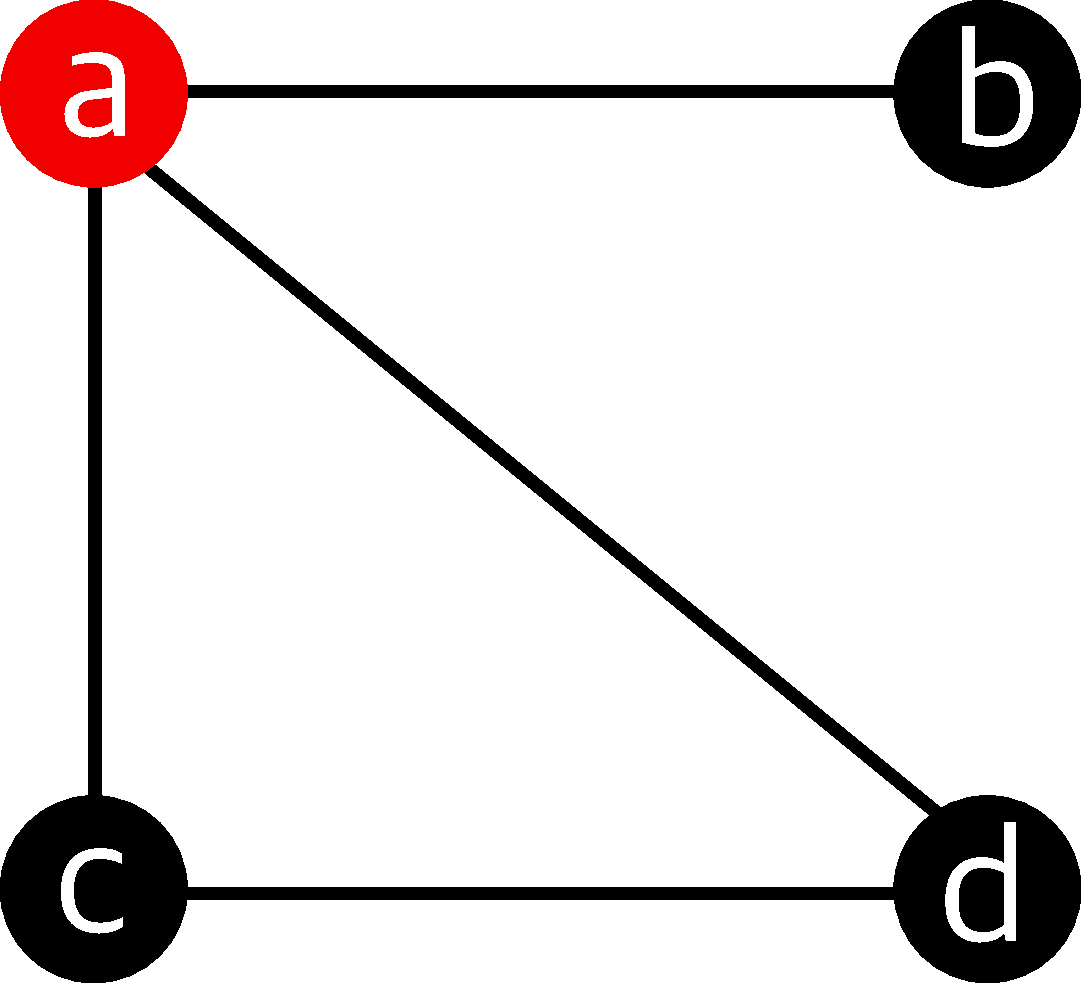
\includegraphics[width=\textwidth]{figures/diff2vec1}
  \caption{Subgraph $\tilde{G}$}
  \end{subfigure}
  \hfill
  \begin{subfigure}[b]{0.4\linewidth}
  \centering
  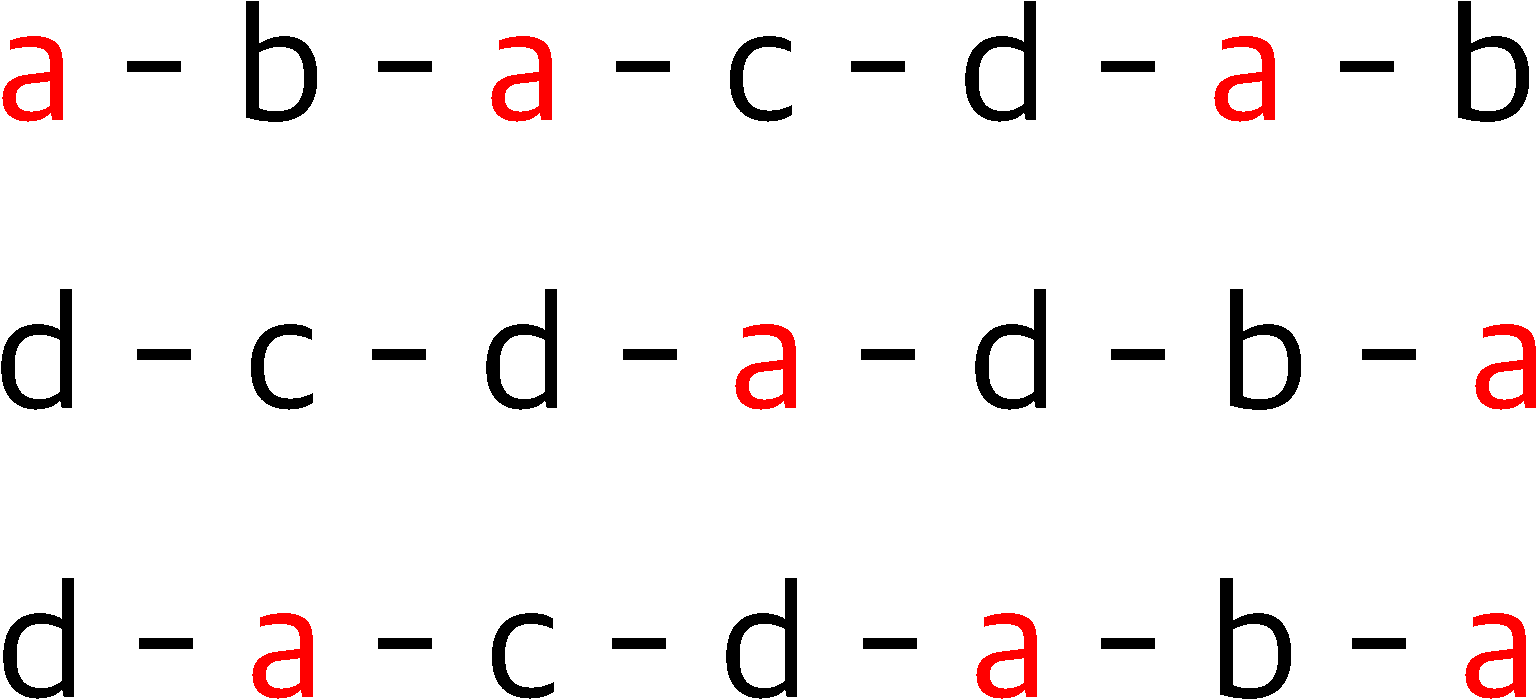
\includegraphics[width=\textwidth]{figures/diff2vec2}
  \caption{Sequences $S$}
  \end{subfigure}
  \hfill
  \par\bigskip
  \hfill
  \begin{subfigure}[b]{0.4\linewidth}
  \centering
  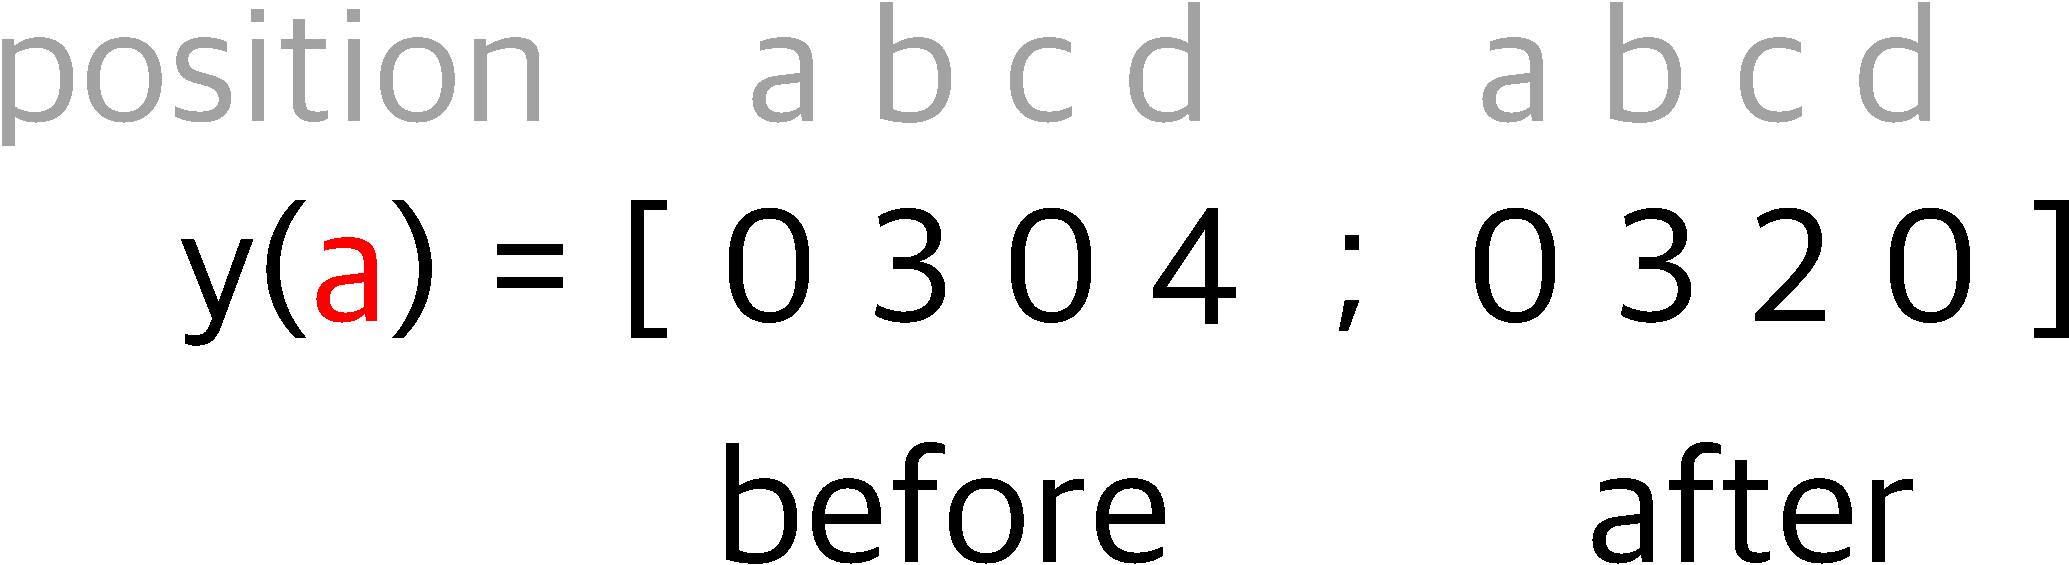
\includegraphics[width=\textwidth]{figures/diff2vec3}
  \caption{Feature $y(a)$}
  \end{subfigure}
  \hfill
  \begin{subfigure}[b]{0.4\linewidth}
  \centering
  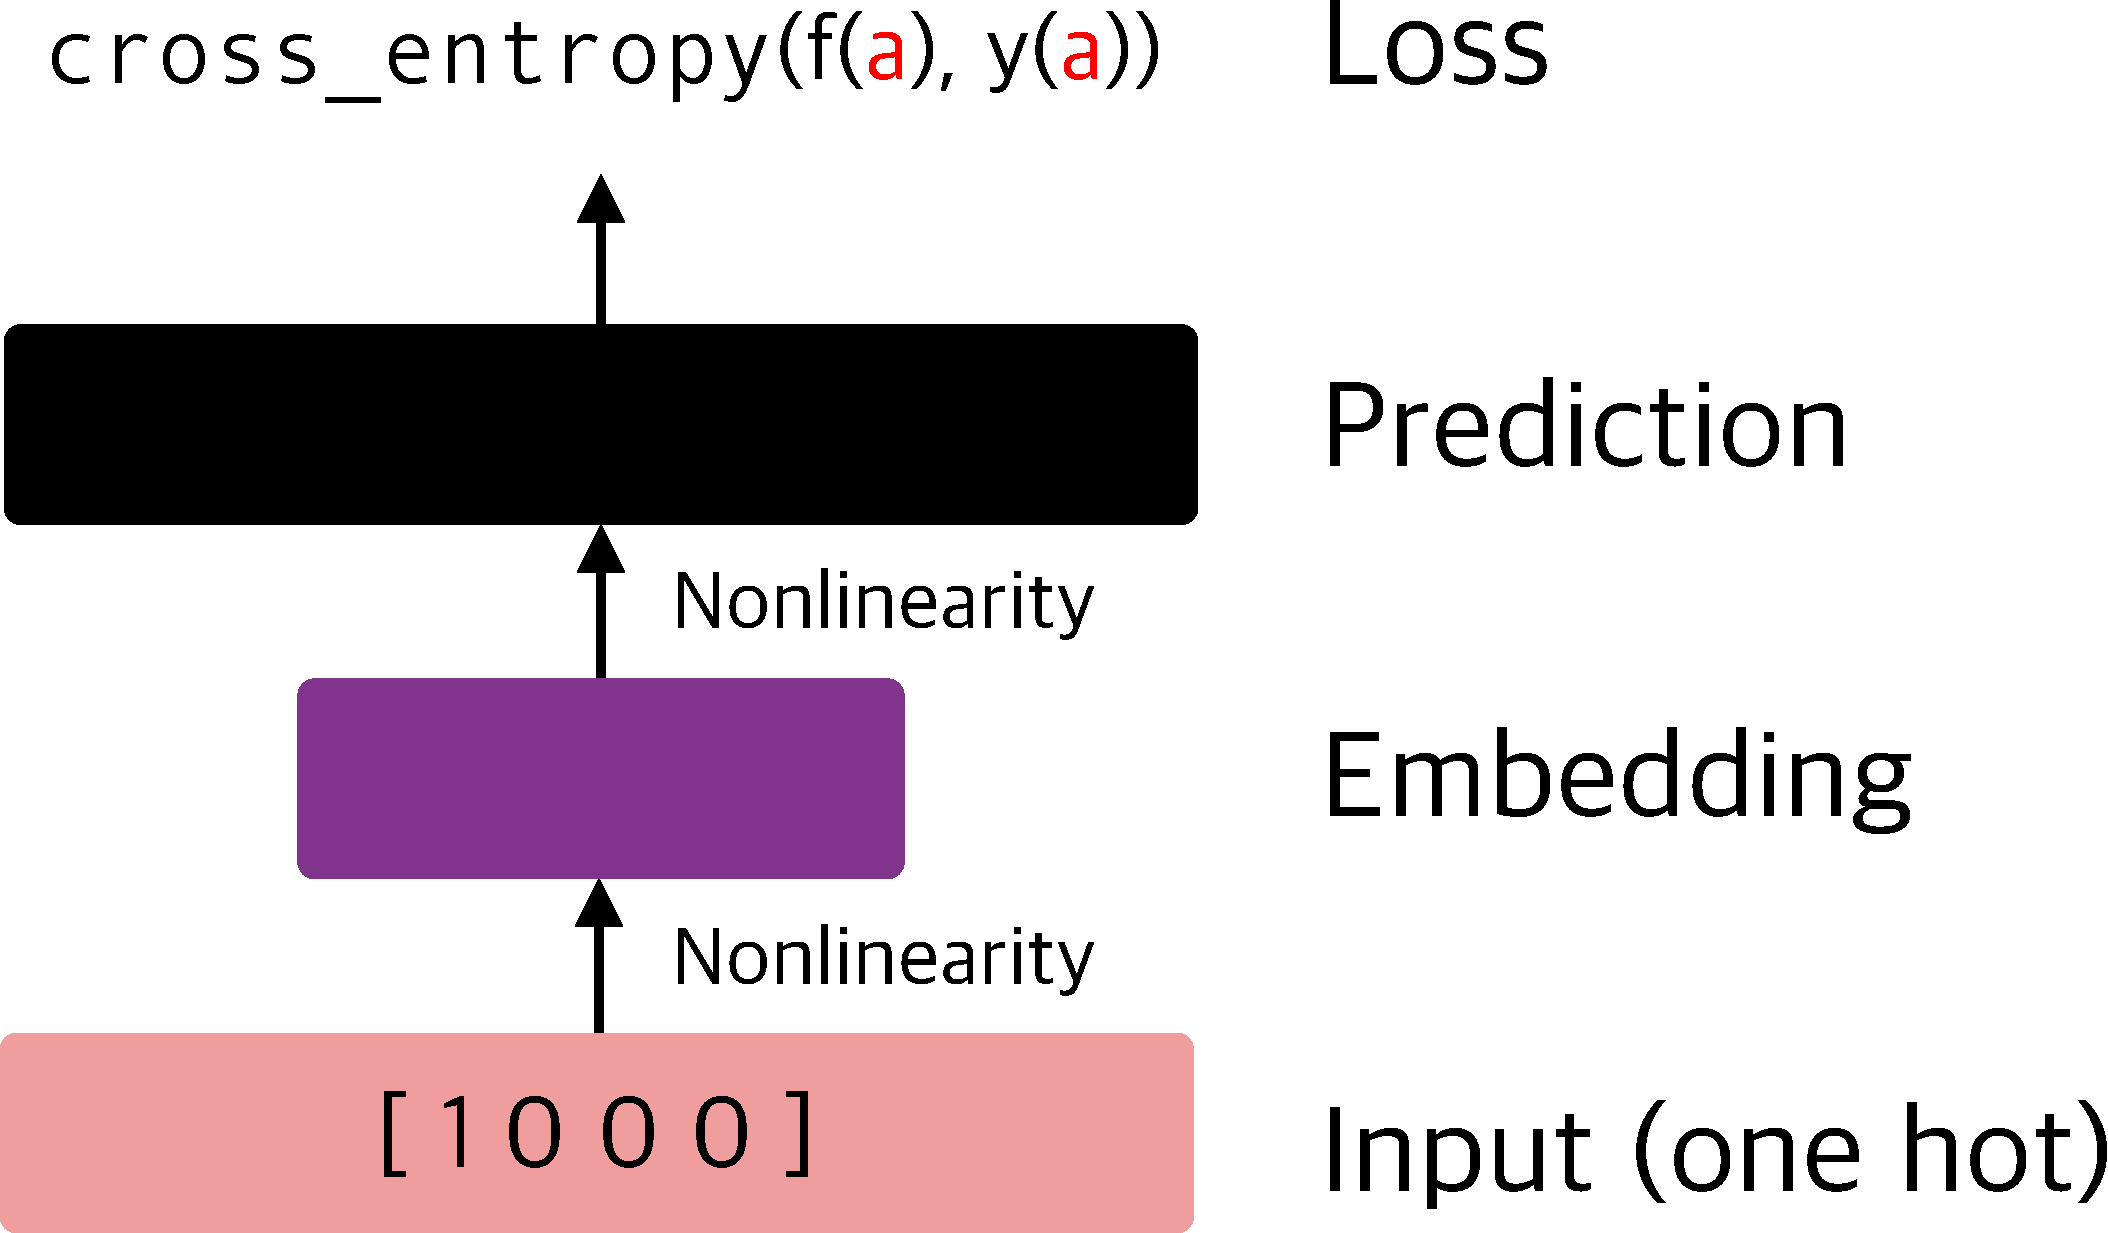
\includegraphics[width=\textwidth]{figures/diff2vec4}
  \caption{Word2Vec $f_\theta$}
  \end{subfigure}
  \hfill
\caption{The four steps of the Diff2Vec algorithm, focusing on the individual node $a \in V$.}
\label{fig:diff2vec}
\end{figure}

Steps three and four amount to Word2Vec\footnote{We use \texttt{gensim.models.word2vec}.} \citep{mikolov2013efficient,mikolov2013distributed}. In practice we optimize with SGD for 5 epochs with a learning rate of 0.025. We set $d = 128$, $l = 40$, and $h = 5$. Given an address $v \in V$, to find its cluster, we can search for the closest $k$ vectors in $\mathbb{R}^d$. In practice, we accomplish this efficiently using FAISS \citep{johnson2019billion}. Unlike DAR, this heuristic will always return $k$ addresses. We score the confidence of an address $u$ in the cluster by the inverse of its Euclidean distance to the embedding of $v$:
\begin{equation*}
\kappa(u) = \frac{1}{\|f_\theta(\texttt{one\_hot}(u)) - f_\theta(\texttt{one\_hot}(v))\|_2}
\end{equation*}
since a smaller distance (closer to 0) represents more semantic similarity of $u$ to $v$.

\subsection{Anonymity Score}
\label{sec:anonymityscore}

Given a query address $v$, using one or both heuristics, we obtain a set of clustered addresses $C$ with confidence scores $\kappa$ for every member. We wish to compute a statistic summarizing the anonymity of the query address, such that a larger cluster reveals more identity information, hence lower anonymity. We define the anonymity score as:
\begin{equation}
\texttt{anonymity}(v) = 1 - \texttt{tanh}(\beta * \kappa(v) * |C|)
\label{eq:anonymity}
\end{equation}
where $\beta$ is a hyperparameter controlling slope. A larger value for $\beta$ more aggressively penalizes larger clusters. We chose $\beta = 0.1$. This anonymity score is a summary statistic representing how easily connected an address is to other addresses potentially owned by the same entity.
% \istvan{$\kappa(v)$ is taken for every node in the cluster?}